\documentclass[a4paper,11pt]{report}

%%%%%%%%%%%%%%%%%%%%%%%%%%%%%%%%%%%%%%%%%%%%%%%%%%%%%%%%%%%%%%%%%%%%%%%
% Definicion de paquetes
\usepackage[T1]{fontenc}
\usepackage[utf8]{inputenc}
\usepackage[spanish]{babel}
\usepackage[printsolution=true]{exercises}
\usepackage[doublespacing]{setspace}% just to set the samples further apart
\usepackage[colorinlistoftodos,prependcaption,textsize=tiny]{todonotes}
%%%%%%%%%%%%%%%%%%%%%%%%%%%%%%%%%%%%%%%%%%%%%%%%%%%%%%%%%%%%%%%%%%%%%%%
% Definición de comandos
\setlength{\marginparwidth}{2cm}
\newcommand{\unsure}[2]{\todo[linecolor=red,backgroundcolor=red!25,bordercolor=red,#1]{#2}}
\newcommand{\change}[2]{\todo[linecolor=blue,backgroundcolor=blue!25,bordercolor=blue,#1]{#2}}
\newcommand{\info}[2]{\todo[linecolor=OliveGreen,backgroundcolor=OliveGreen!25,bordercolor=OliveGreen,#1]{#2}}
\newcommand{\improvement}[2]{\todo[linecolor=Plum,backgroundcolor=Plum!25,bordercolor=Plum,#1]{#2}}
\newcommand{\thiswillnotshow}[2]{\todo[disable,#1]{#2}}
\newcommand*{\SignatureAndDate}[1]{%
    \par\noindent\makebox[2.5in]{\hrulefill} %\hfill\makebox[2.0in]{\hrulefill}%
    \par\noindent\makebox[2.5in][l]{#1}      %\hfill\makebox[2.0in][l]{Date}%
}%
%%%%%%%%%%%%%%%%%%%%%%%%%%%%%%%%%%%%%%%%%%%%%%%%%%%%%%%%%%%%%%%%%%%%%%%
%% Empieza el documento
\begin{document}
	\title{Práctica 5 - Individual}
	\author{
		Miguel Emilio Ruiz Nieto
	}

	\maketitle

  \section*{Ejercicio 3}

  % Hablar sobre el resultado de la última propiedad, que da un contraejemplo
  La propiedad ``Nunca nadie con entrada va a los recreativos'' no se satisface
  debido a que da un contraejemplo. El motivo es que sí que es posible ir a los
  recreativos con entrada ya que se puede comprar la entrada, ponerse en la
  cola y no entrar porque o bien el aforo esté completo o bien porque no seas
  mayor de edad, y te echen a la Plaza Mayor. Una vez allí, el sistema permite
  ir a los recreativos con la entrada comprada, por tanto, el hecho de que la
  propiedad no se cumpla es un comportamiento correcto, como se muestra en la
  siguiente figura:
  \begin{figure}[h]
    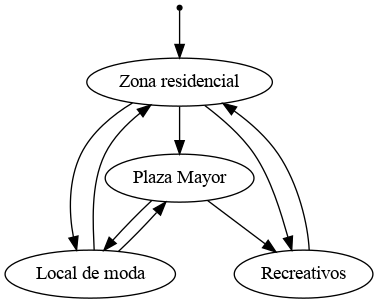
\includegraphics[scale=0.5]{lugares.png}
    \centering
    \caption{Flujo de las personas genéricas en el sistema}
  \end{figure}

  \section*{Ejercicio 4}
  % Hablar sobre las reglas que no pueden convertirse en ecuaciones
  % indicando los motivos, así como las que sí se pueden
  Para poder transformar reglas en ecuaciones, aquellas reglas que se deseen
  transformar han de cumplir que sean terminantes y deterministas, es decir, no
  han de formar bucles y deben confluir siempre en un solo estado, respectivamente.

  Partiendo de esta idea, en el sistema que ha sido definido hay reglas que
  no podrán ser convertidas a reglas porque no cumplen las propiedades, como
  son las reglas de \texttt{hacer-cola-local-de-moda}, \texttt{hacer-cola-local-de-moda-2},
  \texttt{ir-a-recreativos-desde-pza-mayor} y \texttt{volver-a-plaza-mayor}, puesto
  que estas reglas forman un bucle en el cual una persona genérica puede estar
  infinitamente pasando de un lugar a otro. Tampoco lo serían las reglas de
  \texttt{ir-a-plaza-mayor} ni \texttt{ir-a-recreativos} puesto que junto a la
  regla de \texttt{hacer-cola-local-de-moda-2} hacen que no sea deterministas, ya
  que desde la zona residencial se puede ir o a la plaza mayor, al local de moda
  o a los recreativos. Las otras reglas que tampoco cumplen las propiedades son
  \texttt{cruzarse-ebrio-con-bokencio} y \texttt{volver-a-casa-cansado-pero-contento},
  y \texttt{jugar-a-dobles}.

  Ahora bien, una regla que sí podría convertirse en ecuación es la de
  \texttt{entrar-local-de-moda}, puesto que es una regla que no forma bucles,
  luego cumple que sea terminante, y adicionalmente es determinista, porque
  se transita a otro estado bajo las condiciones de que la persona que quiera
  entrar tenga entrada, sea mayor de edad y el aforo del local no esté completo.
  Otras reglas que podrían ser convertidas a ecuaciones son las de \texttt{beber-copa},
  \texttt{beber-refresco} y \texttt{bokencio-bebe-refresco}. Las otra regla que
  también cumple con las propiedades de ser determinista y terminante es la
  de \texttt{comprar-entrada}.

\end{document}